\section{Realizzazione}
Per la realizzazione del sito si è fatto riferimento ad alcune linee guida che ci hanno permesso di impostare il lavoro fin da subito, permettendo una scrittura agevole e relativamente semplice del codice.

\subsection{Responsive Design}
TV Hunter è stato sviluppato con un approccio \textbf{mobile first} responsive.\\
Sono presenti tre breakpoint che permettono una visualizzazione di qualità delle pagine da tutti i tipi di dispositivi comunemente usati per la navigazione.\\
I breakpoint, indicati con l'intera \textit{media query}, sono i seguenti:
\begin{itemize}
	\item \textbf{@media screen and (min-width: 751px) and (max-width: 1024px)} delimita la modalità tablet. Adatta a schemi medio-grandi di tablet o a schermi grandi di smartphone.
	\item \textbf{@media screen and (min-width: 1025px)} delimita l'inizio della modalità desktop. 
\end{itemize}
Lo stile per i dispositivi mobili con larghezza massima di 750px è specificato all'esterno di media query, questà è una caratteristica del codice mobile first.\\
È presente una ulteriore media query per la modalità di stampa.
\subsubsection{Layout di stampa}
Per permettere all'utente di stampare pagine del sito è stato definito un layout di stampa che elimina dalla pagina elementi non utili alla stampa.\\
Ad esempio non sono visualizzati l'header, la barra di navigazione superiore ed inferiore. Gli sfondi scuri sono sostituiti dal colore bianco e i testi sono convertiti in colore nero. Le miniature delle serie TV non sono visualizzate nelle pagine di \textit{esplora} e \textit{preferiti} per evitare il consumo eccessivo di colore in fase di stampa.

\subsection{Linguaggi e strumenti}

\subsubsection{HTML 5}
Abbiamo scelto di utilizzare lo standard HTML 5, il quale include delle direttive per scrivere codice HTML che viene processato come XML. Questo per permettere di avere un aggiornamento futuro del sistema  semplice e sempre al passo con le tecnologie web moderne.

\subsubsection{PHP}
PHP è stato utilizzato per la creazione dinamica di tutte le pagine della piattaforma. Infatti viene generato del codice HTML per ogni pagina in due modi, dalla lettura di un file .txt univoco per ogni pagina e dall'immissione di parti di HTML templetizzate per tutte le pagine in corrispondenza di flag specifici. Il forte utilizzo di PHP ha permesso un interazione tra gli utenti registrati e gli amministratori attraverso \textit{form} per il supporto e per la segnalazione di contenuti presenti nella piattaforma. Inoltre ha permesso di effettuare il caricamento di contenuti preferiti personalizzati per ogni utente e il caricamento della \textit{navbar} personalizzata a seconda della tipologia di utente. 

\subsubsection{JavaScript}
JavaScript è stato utilizzato per l'aggiornamento in tempo reale della pagina web, tramite Ajax. Questo ha permesso di avere aggiornamenti della pagina senza dover effettuare il ricaricamento. Ajax è stato utilizzato nella parte di ricerca della serie, \textit{searchbar}, e nella pagina specifica delle serie dove vengono caricate, se richieste dall'utente, le varie stagioni. Qualora JavaScript non fosse disponibile sono state implementate delle funzioni della parti di PHP che permettono comunque il funzionamento del sito.

\subsubsection{Struttura}
Tutta la parte strutturale è stata mantenuta nei file presenti all'interno della cartella \textit{public}. I files .php invece dentro la cartella \textit{php}. La parte di presentazione invece è stata posta all'interno della cartella \textit{css}, le immagini all'interno della cartella \textit{img}, mentre tutti gli altri file di utilità sono stati posti in cartelle più specifiche. La struttura scelta dal gruppo è quella gerarchica, in quanto tutte le informazioni sono disponibili a partire da una barra di navigazione sempre visibile.

\subsubsection{Database}

Il sito ha un database contenente  sedici tabelle che vengono utilizzate per immagazzinare  tutte le informazioni contenute nel sito e le possibili interazioni da parte degli utenti registrati, come il commentare o votare una serie, spedire un messaggio agli admin ecc. Nell'immagine che segue è illustrata la  sua struttura e le connessioni che sono presenti tra le tabelle:

\begin{figure}[H]
	\centerline{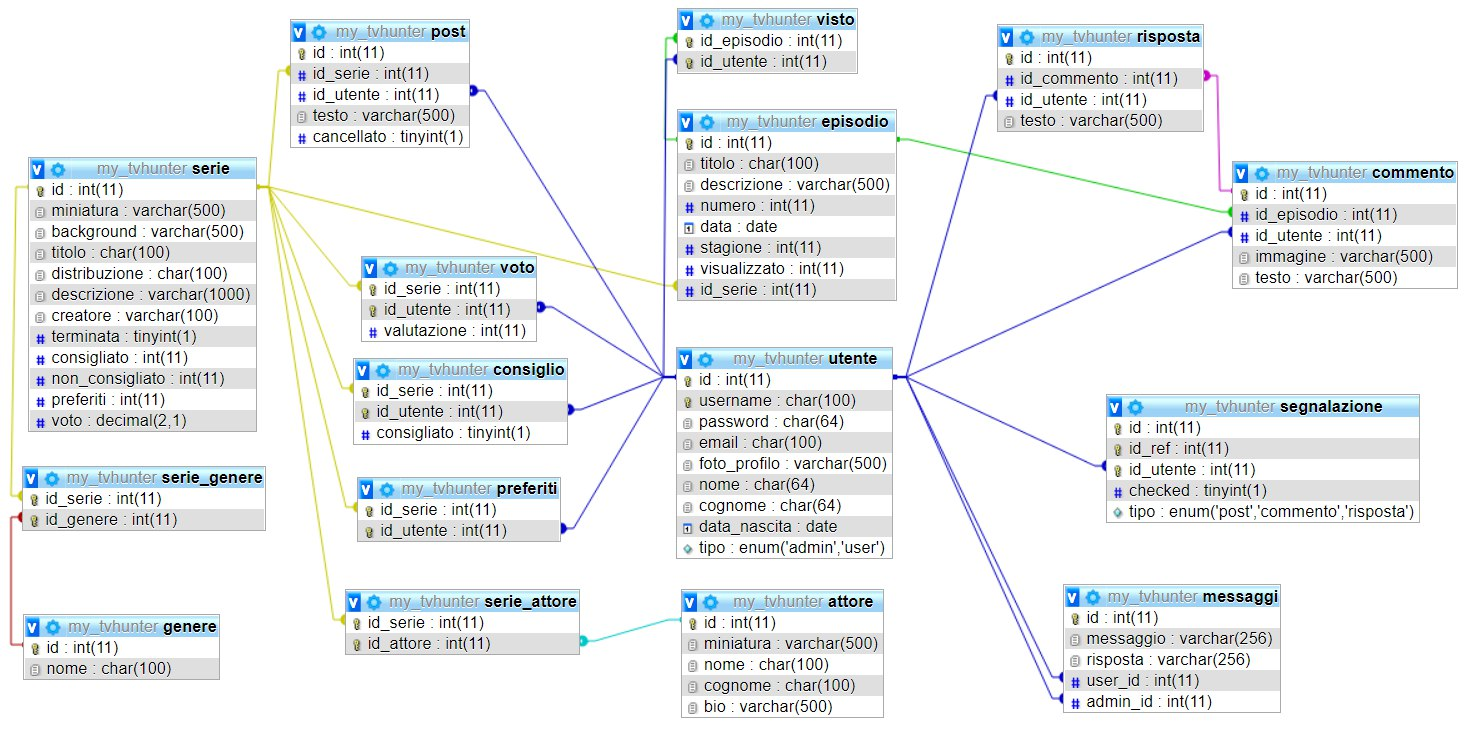
\includegraphics[scale= 0.40]{img/database.jpg}}
	\caption{Database di Tv Hunter}
\end{figure}

Ogni tabella presenta almeno un campo chiave per ogni tipo di dato immagazzinato al suo interno, questo permette di non avere contenuti duplicati ed evita quindi la ridondanza tra dati.

\subsection{Presentazione}
Si è cercata, e ottenuta, una completa separazione tra parte presentazionale e parte strutturale. Non sono presenti \textit{tag} di stile all’interno dell'HTML che viene generato in PHP e nemmeno nei file delle pagine in formato .txt che vengono tradotti in codice HTML. 
Tutta la presentazione viene gestita attraverso fogli di stile diversi che si adattano, come descritto nel paragrafo 3.1, al tipo di dispositivo usato.

\subsection{Comportamento}
Sia per l'utente generico che per l'amministratore si è deciso di utlizzare sia elementi di JavaScript che di PHP, questa scelta è dovuta al fatto che il sito cerca il più possibile di coinvolgere l'utente a commentare e valutare i contenuti, ispirandosi quindi al modello dei social network. È stata inoltre predisposta la validazione degli input da parte dell’utente, con una gestione degli errori per la registrazione nel sistema. Si è scelto di adottare un sistema anti-SQL Injection per la compilazione dei form presenti nel sito in modo da prevenire l'accesso ai dati sensibili. Inoltre sono stati effettuati dei controlli sull'input attraverso la variabile \textit{pattern} presente in HTML nel client-side e per essere certi della validità dell'input sono stati effettuati dei controlli anche dal lato server tramite PHP.


